\section{Experimental Evaluation}
\label{sec:eval}
This evaluation reports one integrated pipeline execution. It contains
separate evidence blocks for workflow coverage, protocol acquisition and
write guards, fixed-seed simulator objectives, and a scripted BOPET task.
These blocks were recorded in the same execution but do not form one
continuous process trajectory or a matched comparison.

\subsection{Run Design and Conditions}
\label{sec:eval-protocol}
The run exercised the configured task-to-device path in deterministic local
simulators. A deterministic tool adapter invoked platform operations; the
language-model loop was disabled. The platform and simulator were already
running, and the run reused shared platform data, so the evaluation does not
measure cold-start commissioning. The run identifier, command, source commit,
and selected records are listed in Supplementary File~S6.

All 17 phase gates passed. At check level, 76 of 77 checks passed, one warned,
and none failed. The warning was the BOPET semantic-card check in phase P10;
the phase gate passed. Table~\ref{tab:workflow-coverage} groups the recorded
checks by workflow block. The grouped checks indicate which configured paths
were exercised; they are not independent system repetitions.

\begin{table*}[!t]
\centering
\caption{Workflow coverage recorded during the integrated pipeline
execution. Check counts are pass/warn/fail; all 17 phase gates passed.}
\label{tab:workflow-coverage}
\footnotesize
\setlength{\tabcolsep}{5pt}
\begin{tabularx}{\textwidth}{@{}>{\raggedright\arraybackslash}p{0.36\textwidth}r r X@{}}
\toprule
Workflow block & Gates & Checks (P/W/F) & Evidence exercised\\
\midrule
Bootstrap, model setup, and scene provisioning & 3 & 11/0/0 & Runtime checks and five-protocol node configuration\\
Acquisition, governed operations, and service records & 8 & 30/0/0 & Sampling, negative probes, approval, recipe, and task routes\\
Seeded objective and multimodal acquisition checks & 2 & 7/0/0 & Three fixed seeds and vector/image acquisition\\
Second-scene configuration and backstop checks & 2 & 16/0/0 & Configuration-only remapping and bounded recovery\\
Platform subsystem checks & 1 & 3/0/0 & Service and registry checks\\
BOPET scene and scripted task & 1 & 9/1/0 & Scene provisioning and three setpoint writes; one semantic-card warning\\
\midrule
Total & 17 & 76/1/0 & No failed checks\\
\bottomrule
\end{tabularx}
\end{table*}

\subsection{Protocol Acquisition and Guarded Operations}
\label{sec:eval-protocol-results}
In the primary cast-film scene, five simulated endpoints exercised Modbus TCP,
Modbus RTU, OPC Unified Architecture (OPC UA), Message Queuing Telemetry
Transport (MQTT), and HTTP.
Five acquisition nodes returned 54 samples. Four endpoints also had
write-control paths. Each received six negative probes, and all 24 probes were
rejected by the configured write-admission checks. Each of the four integration checks logged
one accepted legal write, showing that a permitted request reached its
configured path at least once. Because the run does not retain a complete
positive-control denominator, it does not support a false-block-rate
estimate. Modbus RTU provided acquisition only and is excluded from the write
probe count. On the MQTT endpoint, configuration maps \texttt{linespeed-sp}
to the write node and \texttt{thick} to acquisition; that endpoint returned
six thickness samples and logged one accepted legal-write check. The records
are not paired to estimate a write-to-response effect.

Within the same execution, the second-scene (\texttt{film-line}) configuration
check exercised five endpoints: Modbus TCP, OPC UA, MQTT, Modbus
RTU, and HTTP. They returned 12, 12, 5, 11, and 11 acquisition samples,
respectively (51 total). The three writable routes each logged one accepted
legal write and rejected three negative probes, for 9/9 rejected probes; no
false block or code change was recorded. These are positive-path checks, not a
false-block-rate estimate. This was an in-run configuration check, not an
independent deployment or repetition. Table~\ref{tab:protocol-results}
reports the primary-scene acquisition and write-probe counts; latency summaries
are omitted from the main comparison because event-level timing records and
per-protocol denominators were not retained.

\begin{table}[!t]
\centering
\caption{Acquisition and guarded-write observations from the integrated
run. A recorded legal write is a positive-path check, not a rate estimate.}
\label{tab:protocol-results}
\footnotesize
\setlength{\tabcolsep}{3pt}
\begin{tabularx}{\columnwidth}{@{}>{\raggedright\arraybackslash}p{1.25cm}r r X@{}}
\toprule
Protocol & Samples & Rejected probes & Legal-write record\\
\midrule
Modbus TCP & 9 & 6/6 & One recorded\\
OPC UA & 11 & 6/6 & One recorded\\
MQTT & 6 & 6/6 & One recorded\\
HTTP & 13 & 6/6 & One recorded\\
Modbus RTU & 15 & -- & Acquisition only\\
\bottomrule
\end{tabularx}
\end{table}

\subsection{Fixed-Seed Simulator Objective Cases}
\label{sec:eval-objective}
The pipeline included three fixed-seed objective cases against the simulator's
offline reference $J^*=89.894$. The runner defines $J_{end}$ as the mean of
the last two valid trajectory scores, or as the sole valid score when the
stopping rule ends a case before a second score is available. Table~\ref{tab:integrated-seeds}
also reports $J_{last}$, the final individual trajectory score. The resulting
ratios ranged from 96.3\% to 98.8\% of the reference, with a mean of 97.8\%.
These seed cases belong to the same pipeline execution and are not independent
system-level repetitions.

The simulator score is
$J=55J_{\mathrm{thick}}+25J_{\mathrm{quality}}+8J_{\mathrm{energy}}+7J_{\mathrm{throughput}}$.
The thickness term scores deviation from $50\pm2\,\mu\mathrm{m}$ with soft
degradation outside that band; the quality term reflects defect rate, the
energy term screw speed, and the throughput term line speed. The score is
defined only for melt temperature in $195$--$225\,^{\circ}\mathrm{C}$ and
pressure no greater than $22\,\mathrm{MPa}$.

Seed 43 began inside the configured stopping region and ended with zero
iterations and zero writes. It is therefore a zero-update case, not evidence
of iterative convergence. Seeds 42 and 44 each used two writes. The offline
reference is a simulator benchmark target, not a conventional controller
baseline. Fig.~\ref{fig:objective-ratios} displays the three case-level
ratios without adding a distribution estimate.

\begin{table}[!t]
\centering
\caption{Fixed-seed objective observations from the integrated simulator
run. $J_0$ is the initial score; $J_{end}$ is the mean of the last two valid observations, or the sole
valid observation for an early stop; $J_{last}$ is the final individual
trajectory score.}
\label{tab:integrated-seeds}
\footnotesize
\setlength{\tabcolsep}{2pt}
\begin{tabular}{@{}r r r r r r r r@{}}
\toprule
Seed & $J_0$ & $J_{end}$ & $J_{last}$ & $J^*$ & Ratio & Iter. & Writes\\
\midrule
42 & 66.271 & 88.775 & 88.853 & 89.894 & 98.8\% & 2 & 2\\
43 & 86.542 & 86.542 & 86.542 & 89.894 & 96.3\% & 0 & 0\\
44 & 63.981 & 88.384 & 88.540 & 89.894 & 98.3\% & 2 & 2\\
\bottomrule
\end{tabular}
\end{table}

\begin{figure}[!t]
\centering
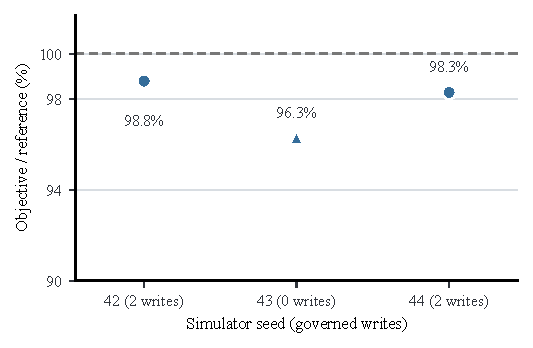
\includegraphics[width=0.96\columnwidth]{resources/fig-objective-ratios-current-run.pdf}
\caption{The three fixed-seed runner-defined end-score ratios ($J_{end}/J^*$)
were 96.3\%--98.8\% of the simulator's offline objective reference. Here
$J_{end}$ is the mean of the last two valid scores, or the sole valid score
when a case stops earlier; $J_{last}$ is the final individual trajectory
score. The dashed line marks 100\%; seed 43 stopped before any update.}
\label{fig:objective-ratios}
\end{figure}

\subsection{Scripted BOPET Integration Trace}
\label{sec:eval-bopet}
A separate task block in the same pipeline execution recorded three setpoint
writes to three distinct controls on a biaxially oriented polyethylene
terephthalate (BOPET) simulator scene. The thickness observations were
28.05, 27.98, 27.98, and $24.84\,\mu\mathrm{m}$, with the final reading inside
the configured $25.0\pm0.7\,\mu\mathrm{m}$ band. This trace demonstrates that the
configured scene and write path produced an in-band simulator observation;
it does not establish that the writes caused the endpoint or that an
optimization was completed. The task-board task reached COMPLETED, while its
associated parameter-change/optimization record remained open and unjudged;
the BOPET phase also contained the single semantic-card warning.
Fig.~\ref{fig:bopet-trace} shows this task separately from the fixed-seed
objective cases.

\begin{figure}[!t]
\centering
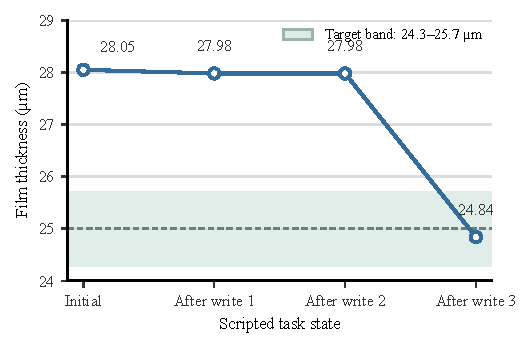
\includegraphics[width=0.96\columnwidth]{resources/fig-bopet-integration-trace.pdf}
\caption{One scripted BOPET task recorded an in-band terminal thickness of
 $24.84\,\mu\mathrm{m}$ after three writes. The shaded area marks the configured
$24.3$--$25.7\,\mu\mathrm{m}$ target band. The task-board task completed; its
associated parameter-change/optimization record remained open and unjudged.}
\label{fig:bopet-trace}
\end{figure}

\subsection{Evidence Boundary}
The run supports a bounded claim that the configured simulator paths connected
five protocol endpoints to data acquisition and that the tested negative
probes were rejected by the configured write guards. The objective ratios and BOPET
trace are separate simulator observations within this run. Because the
language-model loop was disabled, the platform and simulator were already
running, no conventional controller baseline was used, and no physical
equipment was involved, the evidence does not establish autonomous agent
behavior, comparative control benefit, cold-start commissioning, independent
repeatability, or field performance. Post-run hashes verify the delivered
evidence files, not the runtime configuration at execution time.
